
\documentclass[acmsmall,review,anonymous]{acmart}
\settopmatter{printfolios=true,printccs=false,printacmref=false}

%% Remove copyright box
\setcopyright{none}
\renewcommand\footnotetextcopyrightpermission[1]{}
\pagestyle{plain}

\bibliographystyle{ACM-Reference-Format}
\citestyle{acmauthoryear}

\usepackage{newunicodechar}
\newunicodechar{ℕ}{\ensuremath{\mathbb{N}}}

\usepackage{amsthm}
\usepackage{tikz}
\usepackage{appendix}
\theoremstyle{definition}
\newtheorem{definition}{Definition}

\usepackage[references]{agda}

\begin{document}
\begin{code}[hide]%
\>[0]\AgdaKeyword{module}\AgdaSpace{}%
%
%<*AgdaTag-paper>
\AgdaModule{paper}%
%</AgdaTag-paper>
\AgdaSpace{}%
\AgdaKeyword{where}\<%
\\
%
\\[\AgdaEmptyExtraSkip]%
\>[0]\AgdaKeyword{open}\AgdaSpace{}%
\AgdaKeyword{import}\AgdaSpace{}%
%
%<*AgdaTag-Data.Fin>
\AgdaModule{Data.Fin}%
%</AgdaTag-Data.Fin>
\AgdaSpace{}%
\AgdaKeyword{using}\AgdaSpace{}%
\AgdaSymbol{(}%
%<*AgdaTag-Fin>
\AgdaDatatype{Fin}%
%</AgdaTag-Fin>
\AgdaSymbol{)}\<%
\\
\>[0]\AgdaKeyword{open}\AgdaSpace{}%
\AgdaKeyword{import}\AgdaSpace{}%
%
%<*AgdaTag-Data.Nat>
\AgdaModule{Data.Nat}%
%</AgdaTag-Data.Nat>
\AgdaSpace{}%
\AgdaKeyword{using}\AgdaSpace{}%
\AgdaSymbol{(}%
%<*AgdaTag-ℕ>
\AgdaDatatype{ℕ}%
%</AgdaTag-ℕ>
\AgdaSymbol{)}\<%
\end{code}

\title{Formalizing Vector Clocks in Agda (Functional Pearl)}

\author{Gan Shen}
\affiliation{\institution{University of California, Santa Cruz} \country{USA}}
\author{Simon Guo}
\affiliation{\institution{University of California, Santa Cruz} \country{USA}}
\author{Lindsey Kuper}
\affiliation{\institution{University of California, Santa Cruz} \country{USA}}

\begin{abstract}
Distributed systems are hard to build partly because the lack of
physically synchronous global clocks makes reasoning about causality
sometimes impossible. To this end, vector logical clocks have been
proposed and proved to capture causality, in particular, they preserve
and determin the happens-before relation. However, most of the proofs
are done informally on paper.

In this paper...
\end{abstract}

\begin{document}

\maketitle

\section{Introduction}

\section{System Model}
We model a distributed system as consisting of a fixed number of
processes communicating solely by messages. In Agda, we postulate the
number of processes \AgdaRef{n}\footnote{\ensuremath{\mathbb{N}} is
the Agda type of natural numbers.} and the type of the messages
\AgdaRef{Message}\footnote{Set is the Agda type of arbitrary types}:
\begin{code}%
\>[0]\AgdaKeyword{postulate}\<%
\\
\>[0][@{}l@{\AgdaIndent{0}}]%
\>[2]%
%<*AgdaTag-n>
\AgdaPostulate{n}%
%</AgdaTag-n>
\AgdaSpace{}%
\AgdaSymbol{:}\AgdaSpace{}%
%
%<*AgdaTag-ℕ>
\AgdaDatatype{ℕ}%
%</AgdaTag-ℕ>
\<%
\\
%
\>[2]%
%<*AgdaTag-Message>
\AgdaPostulate{Message}%
%</AgdaTag-Message>
\AgdaSpace{}%
\AgdaSymbol{:}\AgdaSpace{}%
\AgdaPrimitive{Set}\<%
\end{code}
In an abstract way, the history of a process can be viewed as a
sequence of events that take place on it, where events are sendings
and receivings of messages. Similarly, the history of one execution of
a distributed system can be viewed as an collection of sequences of
events of each process. We assume each process is assigned an unique
identifier \AgdaRef{ProcessId}\footnote{Fin n is the Agda type of
natural numbers less than n.} and each message is assigned a local
identifier \AgdaRef{LocalEventId} that corresponds to the order it
takes place on its originating process:
\begin{code}%
\>[0]%
%<*AgdaTag-ProcessId>
\AgdaFunction{ProcessId}%
%</AgdaTag-ProcessId>
\AgdaSpace{}%
\AgdaSymbol{=}\AgdaSpace{}%
%
%<*AgdaTag-Fin>
\AgdaDatatype{Fin}%
%</AgdaTag-Fin>
\AgdaSpace{}%
%
%<*AgdaTag-n>
\AgdaPostulate{n}%
%</AgdaTag-n>
\<%
\\
\>[0]%
%<*AgdaTag-LocalEventId>
\AgdaFunction{LocalEventId}%
%</AgdaTag-LocalEventId>
\AgdaSpace{}%
\AgdaSymbol{=}\AgdaSpace{}%
%
%<*AgdaTag-ℕ>
\AgdaDatatype{ℕ}%
%</AgdaTag-ℕ>
\<%
\end{code}
\noindent As as result, we can identify
a event by a product of its originating process's \AgdaRef{ProcessId}
and its \AgdaRef{LocalEventId}.

Events are related, one relation that we are in particular interested
in is Lamport's happens-before relation that establishes an strict
partial order on events:
\begin{definition}[Happens-Before]
  We say event $e$ happens before $e'$ if and only if:
  \begin{enumerate}
  \item $e$ and $e'$ occur on the same process and $e$ takes place before $e'$; or
  \item $e$ is a sending event and $e'$ is the correspoinding receiving event; or
  \item $e$ happens before $e''$ and $e''$ happens before $e'$ for any event $e''$.
  \end{enumerate}
\end{definition}
\noindent Two distinct events $e$ and $e'$ are said to be concurrent
if neither $e$ happens before or $e'$ happens before $e$.  It is
well-known that the happens-before relation captures the potential
causality of events in an execution.

To decide if event $e$ happens before $e'$, one has to position the
two events into a particular history and see if one of the three
conditions of happens-before holds.  This requires us to define
reachable histories, which is traditionally done as a state transition
system.

\section{Strong Clock Condition}

\subsection{Happens-Before Preserving}
As a shorthand, we will refer to the index on the vector clock of an event $e$ that represents $e$'s process as $e$'s process index, i.e. $vc[ e ]$ 's value at $e$'s process index is $vc[ e ] pid[ e ]$.
Then to prove \emph{Happens-Before Determining}, $vc[\_]$ preserves the happens-before partial order between two events

\begin{code}%
\>[0]\AgdaComment{--\ ⊏-preserving\ :\ ∀\ \{pid\ pid′\ eid\ eid′\}\ \{e\ :\ Event\ pid\ eid\}\ \{e′\ :\ Event\ pid′\ eid′\}}\<%
\\
\>[0]\AgdaComment{--\ \ \ \ \ \ \ \ \ \ \ \ \ \ \ \ →\ e\ ⊏\ e′\ →\ vc[\ e\ ]\ ≺\ vc[\ e′\ ]}\<%
\end{code}

We observe that definition of $vc[\_]$.  makes sure that an event always increments its vector clock at its process index.

(insert definition of $vc[\_]$)

From this we can extract the following more  facts, stated more verbosely: 
\begin{itemize}
    \item The vector clock of a send event $send\,m\,e$ is greater than its local preceding event $e$ at their shared process index $pid[ e ]$, and equal to it at every other index. 
    \item The vector clock of a receive event $recv\,e\,e'$ is greater than the maximum $vc[ e ]$ of $vc[ e' ]$ at its process index $pid[ e']$, and equal to it at every other index. This in turns means it's greater than either $vc[ e ]$ of $vc[ e' ]$ at $pid[ e']$ and greater or equal to them at every other index.
\end{itemize}
Then we pattern-match on the happens-before relation,yielding 4 cases corresponding to the constructors of 
$\_\sqsubset\_$. In the first 3 cases ($processOrder_1$,$processOrder_2$, $send\sqsubset recv$), the facts we established earlier tells us that the index where strict greater-holds is exactly the process index of the causally later $e'$, and at every other index $vc[ e' ]$ is either greater than or equal to $vc[ e ]$ as required by. Therefore the requirements for VC greater-than is satisfied. The last transitive case then holds by induction.

\subsection{Happens-Before Determining}
To prove the reverse direction, i.e. an event $e$ happens-before $e'$ only if the vector clock of  $e$ is less than the vector clock of $e'$. 

(insert code for Happens-Before Determining)

we will first prove two lemmas that refine  \emph{Happens-Before Preserving} and \emph{Happens-Before Determining}, by restricting the vector clock comparison to only involve a single index. They split the proof more difficult \emph{Happens-Before Determining} into manageable chunks.

The first lemma refines the 
the VC greater-than relation $\prec$. The VC greater-than only guarantees the existence of a index where the value of is strictly greater. Whereas this lemma makes explicit that, for vector clocks under the holy-grail protocol, this index is exactly the process index of the causally later event. 
\begin{theorem}[Index Happens-Before Preserving]
Let $e$ and $e'$ be two events on arbitrary processes, then $e \sqsubset e'$ implies the vector clock of $e$ is less than the vector clock of $e'$ at $e'$'s index.
\end{theorem}
We first examine the happens-before relation between $e$ and $e'$, and the same 3 cases  ($processOrder_1$,
$processOrder_2$, and $send\sqsubset recv$), $vc[ e ] pid[ e' ] < vc[ e' ] pid[ e' ]$ can be proven with the same facts listed in 2.1, focusing only on $e'$'s process index.

The last transitive case is slightly more tricky as it involves a hidden event $e''$, such that $e''$ happens after $e$ and before $e'$. An example is shown in Figure 1. Using only induction would not suffice since  $e''$ and $e'$'s indices could be different. In this case, we invoke \emph{Happens-Before Preserving} to establish that $vc[ e ] pid[ e' ] \leq vc[ e'' ] pid[ e' ]$, then induction on $e \sqsubset e'$ produces $vc[ e ] pid[ e' ] \leq vc[ e'' ] pid[ e' ] < vc[ e' ] pid[ e' ]$. \qed
\begin{figure}
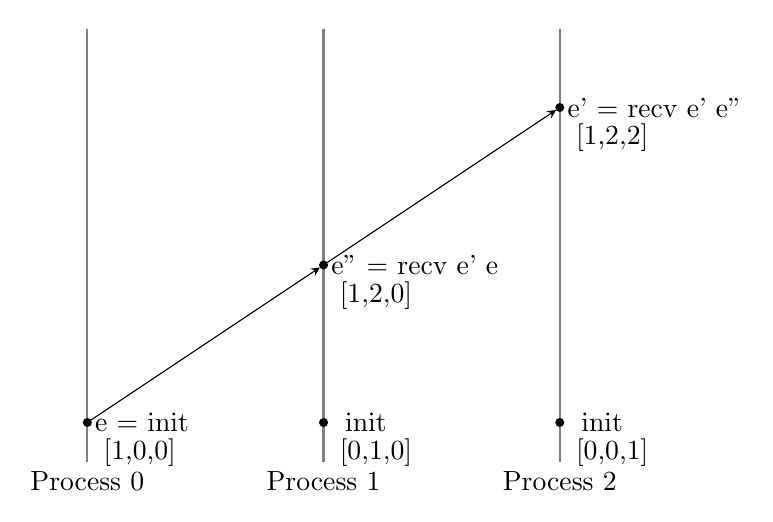
\begin{tikzpicture}
\tikzstyle{every node}=[fill, minimum size = 1pt, inner sep=1pt]
\draw[gray, thick] (-3,3) -- (-3,-2.5);
\draw[gray, thick] (0,3) -- (0,-2.5);
\draw[gray, thick] (3,3) -- (3,-2.5);
\node[shape=circle,draw=black, label=right:{e = init},
label={[label distance=5pt]315:[1,0,0]},
label={[label distance=15pt]below:{Process 0}}
] (e) at (-3,-2) {};
\node[shape=circle,draw=black, label=right:{e'' = recv e' e},
label={[label distance=5pt]315:[1,2,0]}
] (e'') at (0,0) {};
\node[shape=circle,draw=black, label={[label distance=5] right:{init}},
label={[label distance=5pt]315:[0,1,0]},
label={[label distance=15pt]below:{Process 1}}
] at (0,-2) {};
\node[shape=circle,draw=black, label=right:{e' = recv e' e''},
label={[label distance=5pt]315:[1,2,2]}] (e') at (3,2) {};
\node[shape=circle,draw=black, label={[label distance=5] right:{init}},
label={[label distance=5pt]315:[0,0,1]},
label={[label distance=15pt]below:{Process 2}}
] at (3,-2) {};

\draw[-stealth] (e'') -- (e');
\draw[-stealth] (e) -- (e'');

\end{tikzpicture}
\caption{Figure 1}
\end{figure}

The second lemma is a special case of  \emph{Happens-Before Preserving} that operate on separate processes. 

(insert code for Index Happens-Before Preserving)

\begin{theorem}[Index Happens-Before Determining]
Let $e$ and $e'$ be two events on different processes, then $e$ is less than the vector clock of $e'$ at $e$'s index implies $e \sqsubset e'$
\end{theorem}

(insert code for Index Happens-Before Determining)

The premises of this lemma is set up with structural induction on $e'$ in mind. Because $pid[ e' ] \not\equiv pid[ e  ]$. It is often the case that $vc[ e' ] pid[ e ]$ is unchanged from the preceding event, and we can resolve these cases using the inductive hypothesis. In fact, it is only when $e'$ is a $recv$ event of another event $e''$ from $e$ 's process that this convenient induction scheme breaks. In this case, we could rely on the result in our tool box - the total order of events on $e$ and $e''$s shared process. If $e$ happens before or is equal to $e''$ (heterogenously due to our formation of the total order lemma), then we can derive $e \sqsubset e'$. The other case of $e'' \sqsubset e$ is impossible because by
the first lemma, $vc[ e'' ] pid[ e'' ] 
< vc[ e ] pid[ e'' ]$,which contradicts the premise $vc[ e ]pid[ e ] \leq vc[ e'' ] pid[ e'' ]$ \qed.

This lemma gives a $O(1)$ time check for whether an event $e$ happens before another event $e'$ from a different process - if $vc[ e ] pid[ e ] \leq vc[ e' ] pid[ e ]$ then $e \sqsubset e'$ and if $vc[ e' ] pid[ e' ] \leq vc[ e ] pid[ e' ]$ then $e' \sqsubset e$, otherwise $e \| e'$. 

Using the second lemma, we can prove \emph{Happens-Before Determining} rather succinctly.

(insert code for Happens-Before Determining)

we again case split on whether $e$ and $e'$ are from the same process, i.e. $pid[ e ] \equiv pid[ e' ]$. If they are not, then the first condition of the second lemma is satified , $vc[ e ] \prec vc[ e' ]$ implies the second condition $vc[ e ] pid[ e ] < vc[ e' ] pid[ e ]$, therefore we can directly apply our lemma to derive $e \sqsubset e'$. 

Now we assume $e$ and $e'$ are from the same process. In this case, we use the fact that events on the same process form a total order, then either $e \sqsubset e'$, $e \approx e'$, or $e' \sqsubset e$. $e \cong e'$. $e \sqsubset e'$ is our end goal, and the other undesirable cases can be eliminated. If $e \cong e'$,  then we can derive $vc[ e ] \cong vc[ e' ]$ by congruence, meaning all of their indices are equal and contradicting $vc[ e' ] \prec vc[ e ]$. Similarly $e \sqsubset e'$ is also impossible because we can derive $vc[ e' ] \prec vc[ e ]$ by \emph{Happens-Before Preserving}, contradicting the irreflexivity of $\prec$ \qed.

\section{Conclusion}

Vector clocks~\citep{mattern-vector-time, fidge-vector-time, schmuck-dissertation}, blah blah blah.

\bibliography{refs}


\appendix 
\section{Proof of Index Happens-Before Preserving}

\begin{itemize}
    \item If $e'$ is a $send$ event following e, then $e$ and $e'$ are from the same process, and the vector clock is incremented at their shared index.
    \item If $e'$ is a $recv$ event following $e$ or a $recv$ event of $e$ , then the vector clock of $e$ is incorporated through pointwise maximum into the vector clock of $e'$, which then increments its own index 
    \item If $e \sqsubset e'$ by transitivity, and then there is a hidden event  $e''$, such that $e''$ happens after $e$ and before $e'$. Using only induction would not suffice since  $e''$ and $e'$'s indices could be different. In this case, we invoke $\sqsubset-preserving$ to establish that $vc[ e ] pid[ e' ] \leq vc[ e'' ] pid[ e' ]$, then recursion on $e \sqsubset e'$ gives us $vc[ e ] pid[ e' ] \leq vc[ e' ] pid[ e' ]$. 
\end{itemize}

\section{Proof of Index Happens-Before Determining}

\begin{itemize}
    \item If $e'$ is a $init$ event - recall that the vector clock of an event starts from 0 in all but its own index, which is incremented to 1. Given $e$ and $e'$ are from different processes, we know $vc[ e' ] pid[ e ] \equiv 0$, and the second premise then becomes $vc[ e ] pid[ e ] \leq 0$. However, the vector clock of e starts from 1 at its own in index never decreases. Therefore $vc[ e ] pid[ e ] \leq 0$ is impossible. 
    \item If $e'$ is a $send$ of another event $e''$ , then we know its vector clock value at $pid[ e ]$ is unchanged from $e''$, i.e. $vc[ e ] pid[ e ] \leq vc[ e'' ] pid[ e ]$ and by induction $e \sqsubset e''$, then by transitivity $e \sqsubset e''$.
    \item If $e'$ is a $recv$ of events $e''$ following $e'''$, then like before we know the  vector clock value at $pid[ e ]$ is not incremented, and the premise becomes $vc[ e ] pid[ e ] \leq vc[ e'' ] pid[ e ] \sqcap vc[ e''' ] pid[ e ]$. Now consider which of $vc[ e'' ] pid[ e ]$ and $vc[ e''' ] pid[ e ]$ is greater. 
    \begin{itemize} 
        \item If $vc[ e''' ] pid[ e ]$ is greater, then $vc[ e ] pid[ e ] \leq vc[ e''' ] pid[ e ]$, and by induction $e \sqsubset e'''$, and by transitivity $e \sqsubset e'$.
        \item If $vc[ e'' ] pid[ e ]$ is greater, then $vc[ e ] pid[ e ] \leq vc[ e''] pid[ e ]$. We are not sure if $e''$ is from a different process than $e$, so both case need to be considered. 
        \begin{itemize}
            \item If it is different, then by induction $e \sqsubset e''$, and by transitivity $e \sqsubset e'$ as above.
            \item If it is not different, we invoke the local total order of events on the same process. If $e \sqsubset e''$ or $e \cong e''$, then $e \sqsubset e'$ by $send\sqsubset recv$ and transitivity. The last case $e'' \sqsubset e$ is impossible as as applying \emph{Index Happens-Before Preserving} gives us $vc[ e'' ] pid[ e ] < vc[ e ] pid[ e ]$, contradicting the premise.
        \end{itemize}    
    \end{itemize}
\end{itemize}

\end{document}
